\chapter{Future work}
\label{chap:future_work}

\section{Improvements}
Although the current implementation of the networking stack has enough
functionality to be useful in certain applications, there are a lot of
improvements that can be carried out in order to better the project.


\subsection{Wider data-channels between processes and buffers}
One of the main bottlenecks for the throughput is the raw amount of data the
networking stack is working with at any given moment. Currently, the channels in
the SME busses carrying data are only a byte wide, that is, at any given clock,
a process will only have at most 8 bits to work with.
This 1-byte width has been used because it is the most intuitive to work with,
as packet-header fields usually span a factor of 8 bits.\\
Extending the width of the data-channel in the busses might improve the
throughput manyfold, but it might also introduce more logic to the bit-shifting
and masking to parse the headers. Additionally, this change does not only affect
the parsing and the headers, but also the logic in the addressing for storage
in the buffers, as well as, for instance, the checksum calculation.

\subsection{Add external verification tool}
The tests performed and described in chapter \ref{chap:evaluation} on the
current implementation have shown no major nor breaking bugs or errors for
the supported subset of protocols in the internet protocol suite.
Since the existence of undiscovered bugs cannot be ruled out with the
custom-made testing suite, it is better to use an external verification tool in
order to not transfer any wrong implementation-details over to the
test-tools.\\
There are a multitude of ways to TCP/IP implementation with both regards to
bandwidth and throughput, stability, loss, etc.
One such tool is the \texttt{iperf3}, which is a "TCP, UDP, and SCTP network
bandwidth measurement tool"\cite{iperf3}. It is a highly efficient tool for
both performance test, but also verify the correctness of a networking stack.
By introducing iperf3 as a means to test the implementation of the networking
stack, a much better insight of the correctess of the stack can be gained.




\section{New features}
As discussed in chapter \ref{chap:design}, the networking stack is designed
with extensibility in mind, with a separation for the link-, the internet-, and
the transport-layer. Given a protocol following the classic internet protocol
suite 4-layer model, it should be possible to implement this protocol in the
networking stack without major changes to the underlying structure of the whole
codebase.\\
The implementation only supports \gls{udp} in the transport layer, which is
still a great streaming protocol for a multitude of viable scenarios. However,
situations where packet loss or out-of-order data-stream is not acceptable,
\gls{tcp} is the ideal choice of protocol to implement in the stack. With the
ability to share state across sockets in the \texttt{Transport} module, the
parser for the \gls{tcp} header can be implemented, and the out-of-order nature
of the incoming data is already handled in the \texttt{Data In} buffer.\\
Likewise, the newer version of the Internet Protocol, the \gls{ipv6}, is slowly, but
surely, seeing adoption on the internet. Fortunately, the protocol itself is
actually slightly easier to parse compared to its predecessor, the \gls{ipv4}.
For instance, multiple flags from the older \gls{ipv4} header have been moved
into the optional section of the \gls{ipv6}. Furthermore, fragmentation of
\gls{ipv6} packets have been restricted somewhat, and not all hosts are required
to support it\cite{ipv6_proposed}.


\section{Adding a firewall}
\begin{figure*}
\centering
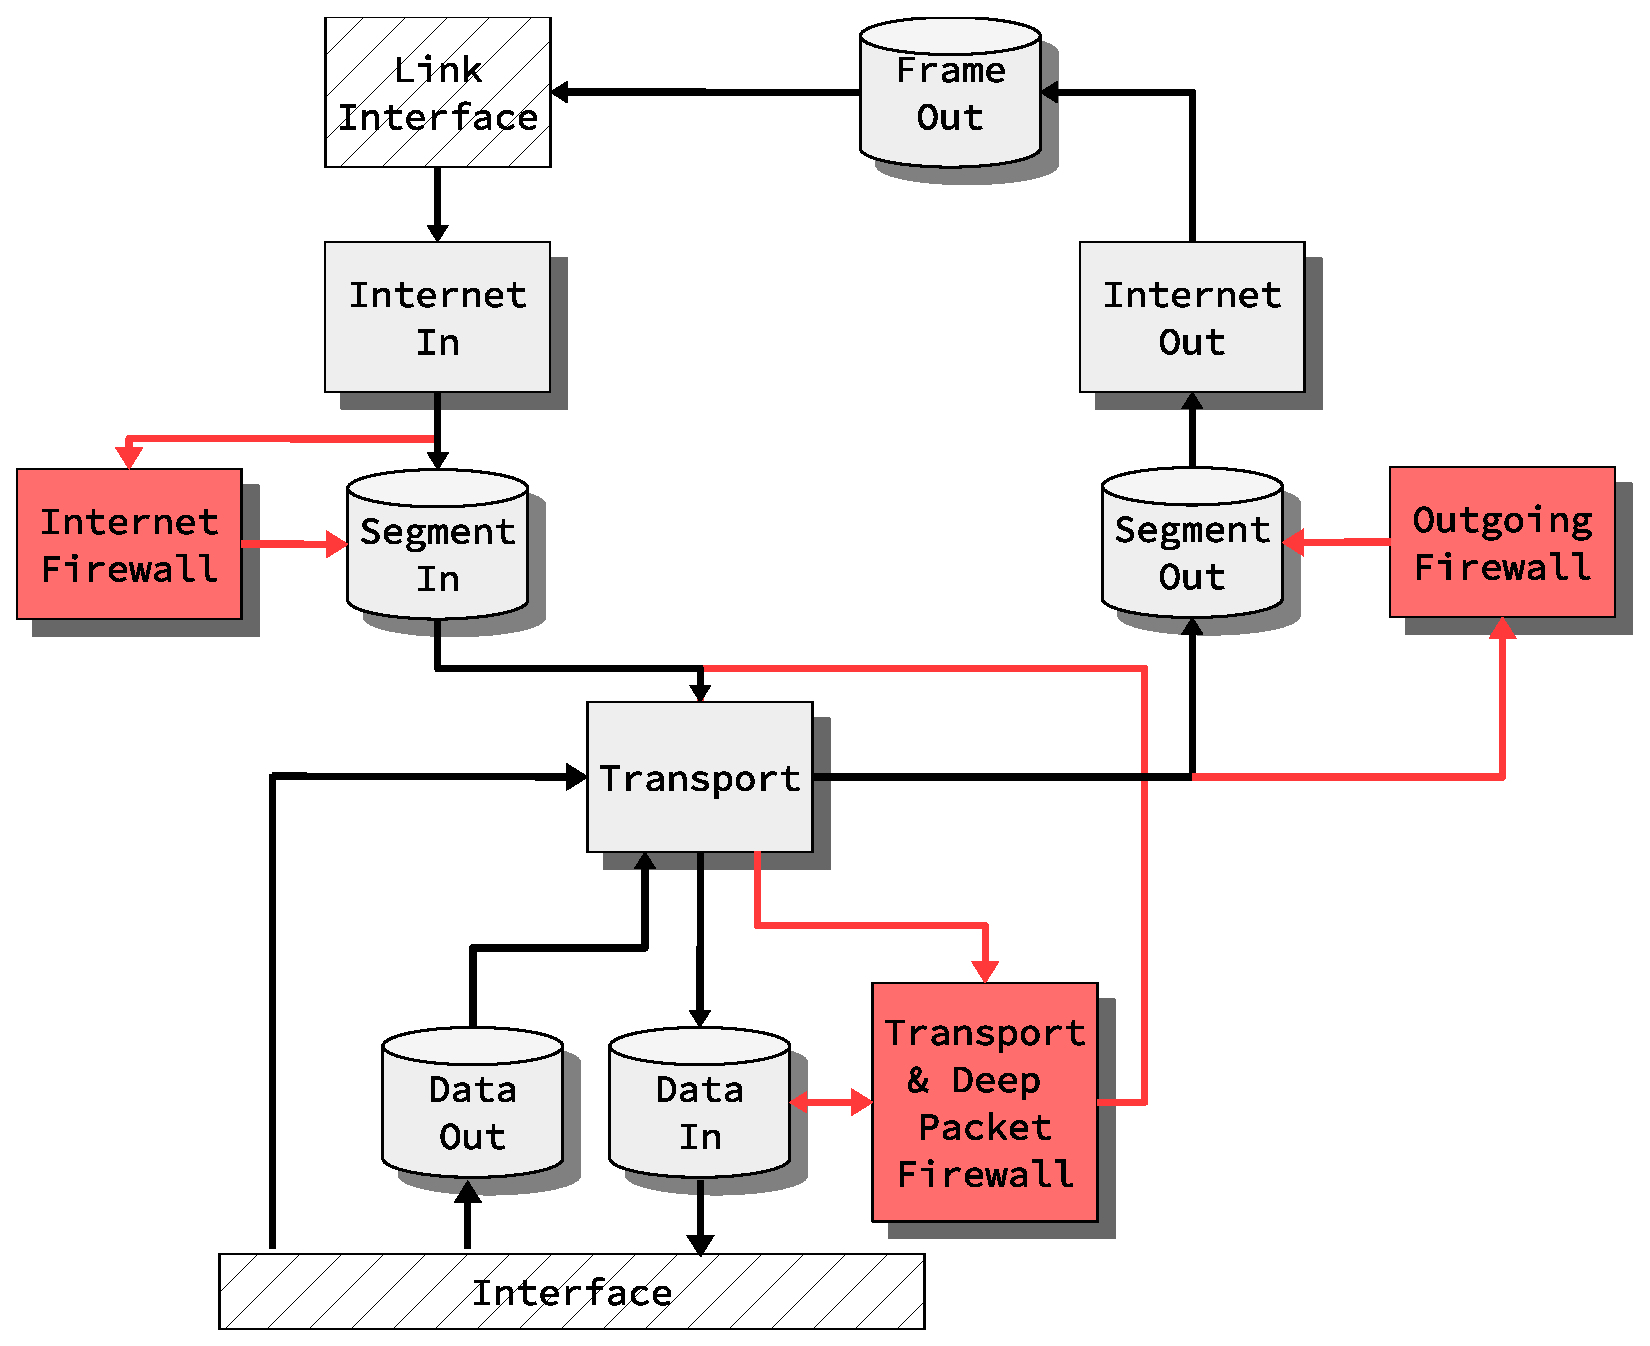
\includegraphics[scale=0.50]{future_work/firewall_integration_design.eps}
\caption{The proposed design for integrating the network stack with the
accompanying firewall}
\label{fig:firewall_integration_design}
\end{figure*}


In tandem with this project, a FPGA firewall has been developed by
Patrick Dyhrberg Sørensen and Emil Sander Bak. Just like the networking stack,
the firewall is implemented in \gls{sme}, with the intent to be easily
integrated with networking stacks, such as this one\cite{fpga_firewall}.\\
The firewall consists of whitelist rules, connection states, "deciding"
processes, and busses for communication and synchronization\cite{fpga_firewall}.\\
The processes making the actual decisions are split into 3 state processe:
\begin{itemize}
\item \textbf{Incoming IPv4}\\
The first point where the firewall can do any decisions is when the internet
protocol header is parsed. This header provides information such as the source
and destination address, and the firewall can do basic checks for blacklisted
or whitelisted addresses, as well as detecting some suspiciously formatted
packets.
\item \textbf{Incoming Transport}\\
The transport-part of the firewall is perhaps a bit more interesting. Here,
the firewall can not only check on the source and destination ports of a packet,
but also verify that there are no malicious intents with regards to the protocol
specification itself. For example, the firewall can detect and stop a SYN-flood
attack, which is a form of \gls{dos attack} where the attacker sends a large
number of TCP SYN-request to a host in order to consume all the host
computational resources.

\item \textbf{Outgoing}\\
The last point that the firewall monitors is the outgoing traffic. This is in
place for situations where the networking stack tries to communicate with
malicious or forbidden hosts.
\end{itemize}

\subsection{Proposal for the design of incorporating the firewall}
Although both projects have been designed to be combined with each other,
there have not yet been any attempts at uniting them.  That being said, both
projects can run self-sufficiently, and all the essential information can
be easily shared across the processes with SME busses.  The proposed design
for incorporation can be seen on figure \ref{fig:firewall_integration_design},
where the parsing processes send information to the firewall, and the firewall
in turn shares its decision with the consequent buffer. This way, the parsing
process has to add all the parsed fields in the bus, and the firewall can mark
the current packet in the bus if it needs to be removed.\\
The main tasks to implement firewall into the networking stack are:
\begin{itemize}
\item \textbf{The bus connection and protocol}\\
The first task is to create the busses for the communication, and to agree on
a signal protocol. Since only one data-transaction with the header info is
needed for each packet, this should not pose a too big of a challenge.

\item \textbf{Connection and packet identification}\\
The networking stack relies on multiple methods of identifying packets.
Once a packet reaches the transport layer, the networking stack can identify
which connection (if any) the packet belongs to. To delimit network-frames, a
frame-number is used, which is supplied by the interface. An \gls{ipv4}
datagram is identified with its \texttt{Identification} header field, and
transport connections are identified by their socket number.
Depending on the implementation of the firewall, there needs to be made an
agreement on the identifiers used to distinguish connections across the
projects.

\item \textbf{Buffer support for packet removal}\\
Apart from the packet itself, the buffer holds additional meta-data used both
by the next parsing layer, but also by the buffer itself to do
de-fragmentation, segmentation, and so on. If a packet is detected to be
malicious by the firewall, a flag should be added to the entry in the buffer to
indicate the removal of it.

\item \textbf{User interface support to control the firewall}\\
It is reasonable to think that the network user would want to control the
firewall live by adding new rules to the white-list, or block certain port
numbers. To simplify this process, new function-calls can be added to the
\texttt{Interface}, and this interface can be connected to the global
state-table in the firewall.
\end{itemize}



